\pdfminorversion=4
\documentclass{beamer}
\usepackage[size=custom,width=121.92,height=91.44,scale=1.4]{beamerposter}
\usetheme{UWMadison}
\usepackage[utf8]{inputenc}
\usepackage{graphicx}
\usepackage{tikz}
\usepackage{mathtools}
\usetikzlibrary{calc}

% formats bibliography
\usepackage[style=phys]{biblatex}
\addbibresource{citations.bib}
\setbeamertemplate{bibliography item}{\insertbiblabel}
\renewcommand*{\bibfont}{\scriptsize}

% formats caption font as well as to not include figure label
\usepackage[font={small,it}]{caption}
\captionsetup{margin=20pt, labelformat=empty}

% adds space between table rows
\usepackage{booktabs}
\renewcommand{\arraystretch}{2.2}
 \newcommand{\lquad}{\hspace{0.5em}} 

\title[small title]{\texorpdfstring{Statistical Methods for Pre-detonation Nuclear Forensics Analysis}
{Statistical Methods for Pre-detonation Nuclear Forensics Analysis}}
\author{Arrielle C Opotowsky, Prof. Paul PH Wilson}
\institute{University of Wisconsin-Madison}
% \date{\today}

\logo{
\includegraphics[height=8cm]{logos/cnerg.png}} % can replace with any other logo (such as DOE, NNSA, etc)
\auspice{ }

\begin{document}
\small

\begin{frame}[t]{}
%\vskip -1cm
\begin{columns}

%%%%%%%%%%%%%%%%%%%%%%%%%%%%%%%%%%%%%%%%%%%%%%%%%%%%%%%%%%%%%%%%%%%%%%%%%%%%%%%%%%%%%%%%%%%%%%%%%%%
\begin{column}[T]{0.27\textwidth}
\begin{block}{Motivation: Speeding up nuclear emergency response}

After a nuclear weapon is detonated or nuclear material is intercepted, a
priority for emergency responders is to determine both where it came from and
the radioactive danger to the public. While the latter can be determined
quickly, the former often involves lab work that can take days or weeks. \\~\\

Attribution of nuclear material is a major part of a nuclear forensics
investigation. This informs both emergency response and what actions the
government takes.  A strong nuclear forensics capability both deters
governments from engaging in state-sponsored nuclear terrorism and interrupts
the pathways being used to create weapons.

\begin{figure}
  \fboxsep=1mm
  \fboxrule=3pt
  \fbox{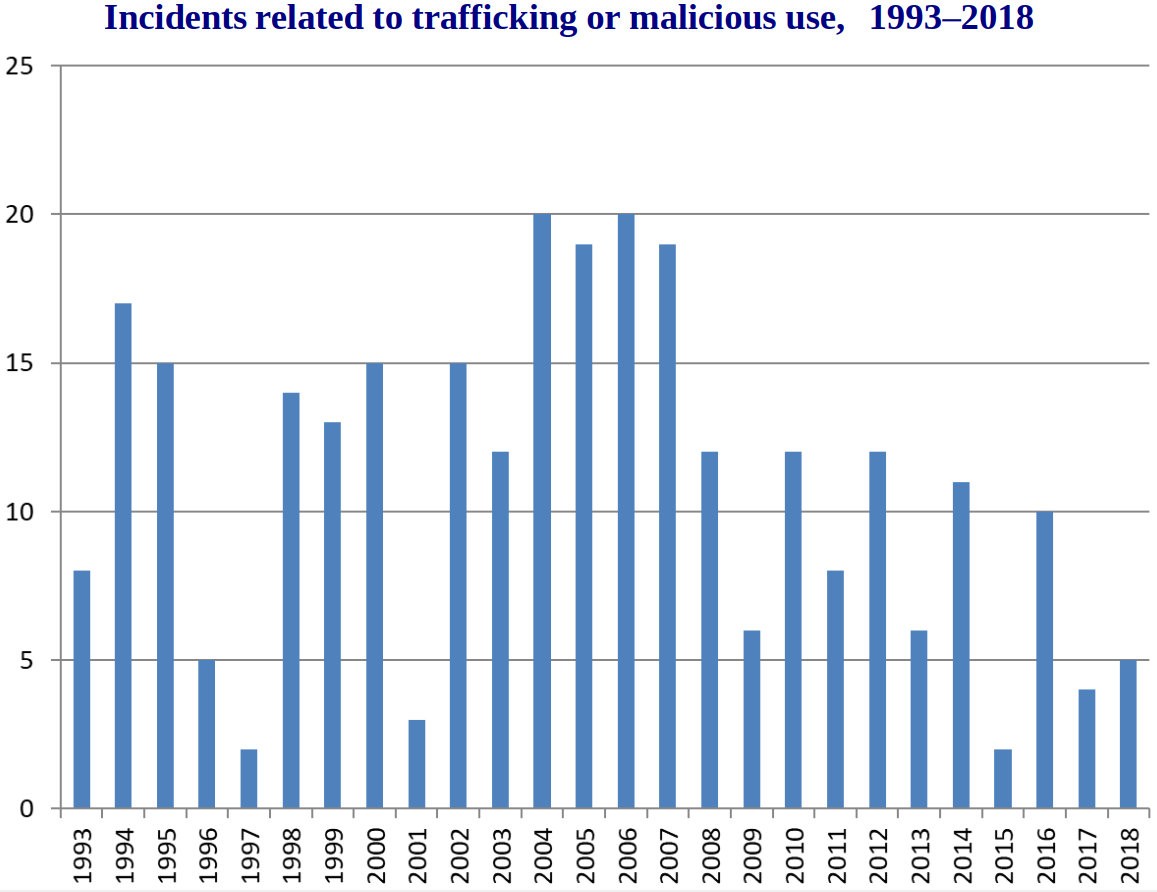
\includegraphics[height=12.5cm]{figures/trafficking.png}}
  \caption{Participating countries (138) report intercepted nuclear materials
           intended for illicit use to the IAEA.\cite{trafficking}}
\end{figure}

The figure shows the number of nuclear material incidents tracked in the last
25 years, of which 12 involved highly enriched uranium, 2 plutonium, and 4
plutonium-beryllium neutron sources.  Thus, this work focuses on spent nuclear
fuel from power reactors outside of regulatory control as a material of
interest. 

\end{block}

\begin{block}{Background: Using statistical methods to evaluate nuclear forensics signatures}

Nuclear forensics research initiatives include characterization of both pre-
and post-detonation materials. Measuring isotopic ratios, chemical compounds,
and trace elements are signatures used to identify the chain of custody of
these materials. Considering spent nuclear fuel, the signatures help determine
a set of reactor parameters that generated the material: reactor type, fuel
enrichment, burnup, and cooling time.  This provides information that can lead
to the source (country, exact reactor) of the material in question.

\begin{figure}
  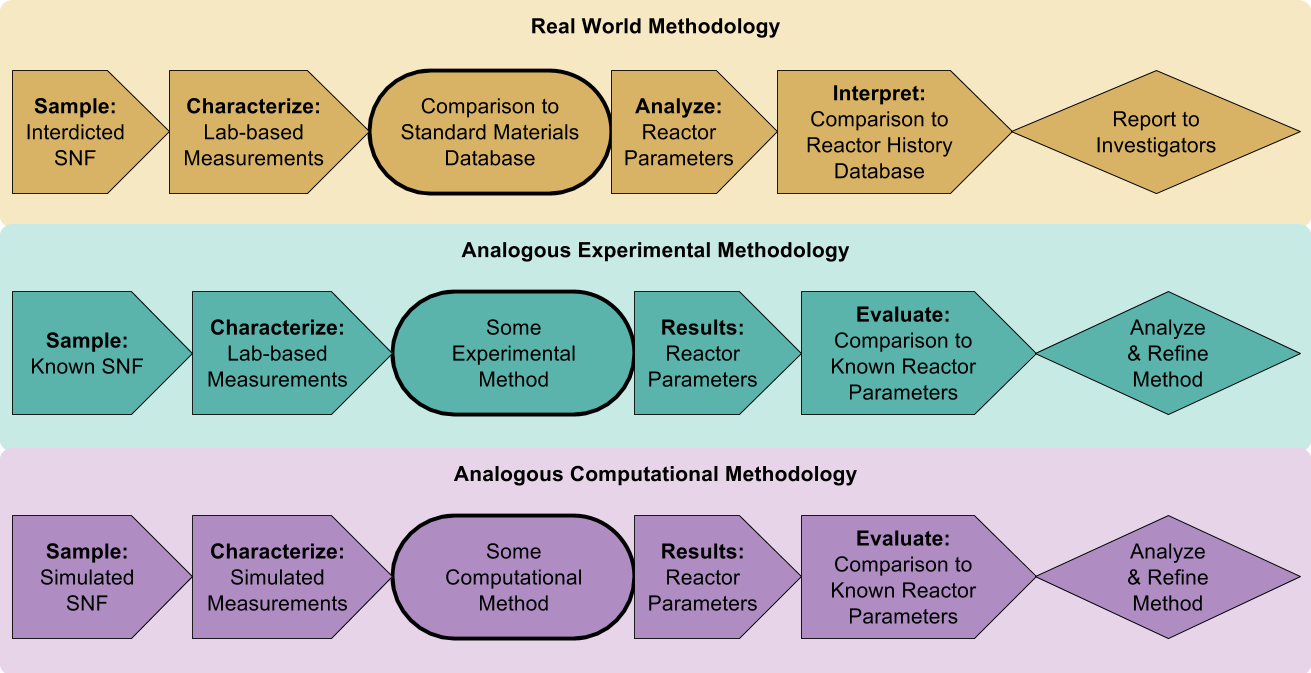
\includegraphics[height=12.5cm]{figures/researchworkflows.png}
  \caption{Nuclear forensics research workflows: physical, experimental, and computational}
\end{figure}

Presented here is a methodology that seeks to rapidly provide
investigation-guiding information using measurements taken in the field
compared against statistical models.  Statistical methods may be able to
determine reactor operation parameters faster than the traditionally utilized
empirical relationships. Shown in the figure is at the top a typical
investigative workflow, followed by an experimental workflow that uses some
method instead of direct comparison to a standard materials database.  This is
extrapolated to a computational method in the bottom panel, which is discussed
further in the methodology sections.

\end{block}
\end{column}
%%%%%%%%%%%%%%%%%%%%%%%%%%%%%%%%%%%%%%%%%%%%%%%%%%%%%%%%%%%%%%%%%%%%%%%%%%%%%%%%%%%%%%%%%%%%%%%%%%%

%%%%%%%%%%%%%%%%%%%%%%%%%%%%%%%%%%%%%%%%%%%%%%%%%%%%%%%%%%%%%%%%%%%%%%%%%%%%%%%%%%%%%%%%%%%%%%%%%%%
\begin{column}[T]{0.72\textwidth}
\begin{columns}[t]
\begin{column}{0.15\textwidth}
\begin{block}{Research Breakdown}

How does the ability to determine forensic-relevant spent nuclear fuel
attributes using machine learning techniques degrade as less information is
available?\\~\\

\begin{figure}
  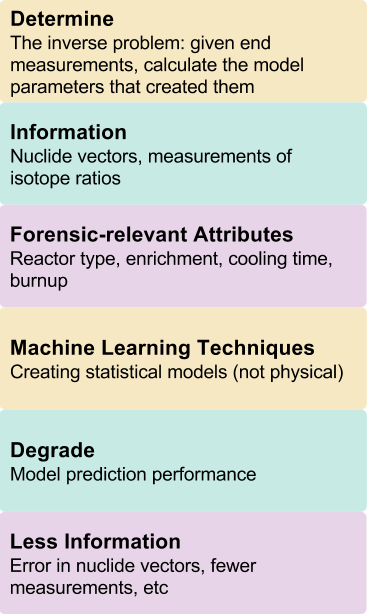
\includegraphics[height=20cm]{figures/overview.png}
  \caption{Definition of terms within the main research question}
\end{figure}

\end{block}
\end{column}

\begin{column}{0.4\textwidth}
\begin{block}{Methodology: Training set creation}

The training set design is based on comparing this workflow to that in previous
work \cite{tamu_method}. The spent nuclear fuel was simulated using Oak Ridge
National Laboratory's ORIGEN \cite{origen}. While this database contains only
three reactors each at a single enrichment, there will be many reactors at
many enrichments added to this database after proof-of-concept is
complete.\\~\\

\begin{minipage}{0.55\textwidth}
\begin{figure}
  
\includegraphics[height=8cm]{figures/mlecompare_inputs.png}
  \caption{Inputs for simulations in training set. The labels include: 
           reactor type, burnup, enrichment, cooling time}
\end{figure}
\end{minipage}%
\begin{minipage}{0.45\textwidth}
\begin{figure}
  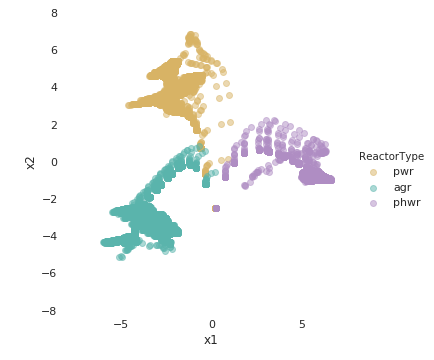
\includegraphics[height=10cm]{figures/lda-trainset.png}
  \caption{Dimensionality reduction step for visualization: 
           linear discriminant analysis of training set can reduce dimensions from 10-15 to 2.}
\end{figure}
\end{minipage}
%\\~\\

\begin{table}
  \begin{tabular}{ |c|c|c|c|c| } 
  \hline
    $\lquad\frac{\prescript{137}{}{Cs}}{\prescript{133}{}{Cs}}\lquad$ & 
    $\lquad\frac{\prescript{134}{}{Cs}}{\prescript{137}{}{Cs}}\lquad$ & 
    $\lquad\frac{\prescript{135}{}{Cs}}{\prescript{137}{}{Cs}}\lquad$ & 
    $\lquad\frac{\prescript{136}{}{Ba}}{\prescript{138}{}{Ba}}\lquad$ &
    $\lquad\frac{\prescript{150}{}{Sm}}{\prescript{149}{}{Sm}}\lquad$ \\
    \hline
    $\lquad\frac{\prescript{152}{}{Sm}}{\prescript{149}{}{Sm}}\lquad$ &
    $\lquad\frac{\prescript{154}{}{Eu}}{\prescript{153}{}{Eu}}\lquad$ & 
    $\lquad\frac{\prescript{240}{}{Pu}}{\prescript{239}{}{Pu}}\lquad$ &
    $\lquad\frac{\prescript{241}{}{Pu}}{\prescript{239}{}{Pu}}\lquad$ & 
    $\lquad\frac{\prescript{242}{}{Pu}}{\prescript{239}{}{Pu}}\lquad$ \\ 
    \hline
  \end{tabular}
  \caption{Features tracked for the training set. This includes 10 isotope ratios
           known to discrimiate the chosen labels well.}
\end{table}

\end{block}
\end{column}

\begin{column}{0.45\textwidth}
\begin{block}{Methodology: Maximum likelihood estimation for prediction}

\begin{figure}
  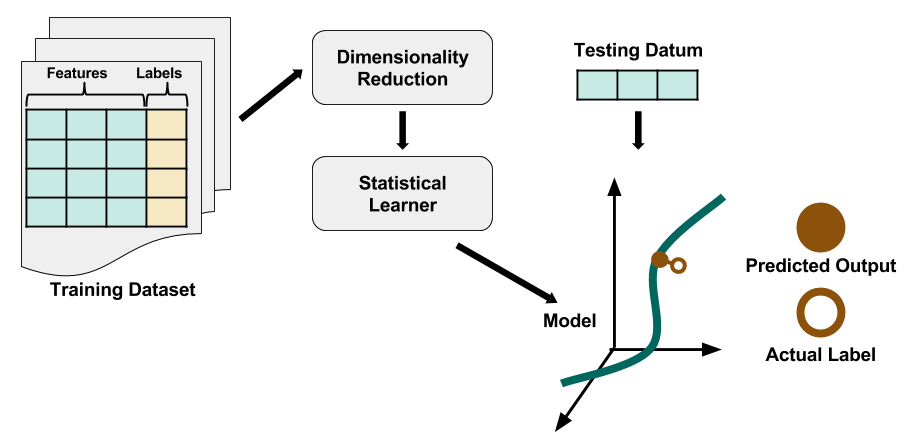
\includegraphics[width=0.68\textwidth]{figures/SupervisedRegression.png}
  \caption{Schematic of a representative training and predicting workflow}
\end{figure}

A generalized machine learning approach for prediction is shown here.  For the
dimensionality reduction step, 200+ isotopes from the simulation were reduced
to 10 isotope ratios. For the statistical learner, a maximum likelihood
estimation (MLE) method was chosen, in part to build upon previous work for this
application. \cite{tamu_method, tamu_sensitivity} \\~\\

Likelihood calculated is as follows:
\[L(M|r_{meas}) = \prod_i \frac{1}{\sigma_{i,sim} \sqrt{2\pi}} \exp{\frac{-(r_{i,meas} - r_{i,sim})^2}{2 \sigma_{i,sim}^2}}\]

%Whereas the log-likelihood is used in practice:
%\[ln(L(M|r_{meas})) = \sum_i ln(\frac{1}{\sigma_{i,sim} \sqrt{2\pi}}) - \frac{-(r_{i,meas} - r_{i,sim})^2}{2 \sigma_{i,sim}^2}\]

A given unknown sample (i.e., testing datum above) with 10 isotope ratios
comprising $\mathbf{r_{meas}}$ will have a likelihood calculated against the
entire training set, each entry containing the ratios $\mathbf{r_{sim}}$ The
prediction is the reactor type entry with the maximum likelihood. The predicted
entry also contains the burnup, cooling time, and fuel enrichment.  An
uncertainty prediction is given from the simulation uncertainty in the isotope
ratios, $\mathbf{\sigma_{sim}}$.

\end{block}
\end{column}
\end{columns}
%%%%%%%%%%%%%%%%%%%%%%%%%%%%%%%%%%%%%%%%%%%%%%%%%%%%%%%%%%%%%%%%%%%%%%%%%%%%%%%%%%%%%%%%%%%%%%%%%%%

%%%%%%%%%%%%%%%%%%%%%%%%%%%%%%%%%%%%%%%%%%%%%%%%%%%%%%%%%%%%%%%%%%%%%%%%%%%%%%%%%%%%%%%%%%%%%%%%%%%
\begin{columns}[t]
\begin{column}{0.6\textwidth}
\begin{block}{Results: MLE Method provides more than just predictions}

Texty text \\~\\

\begin{figure}
\begin{minipage}{.5\textwidth}
  \centering
  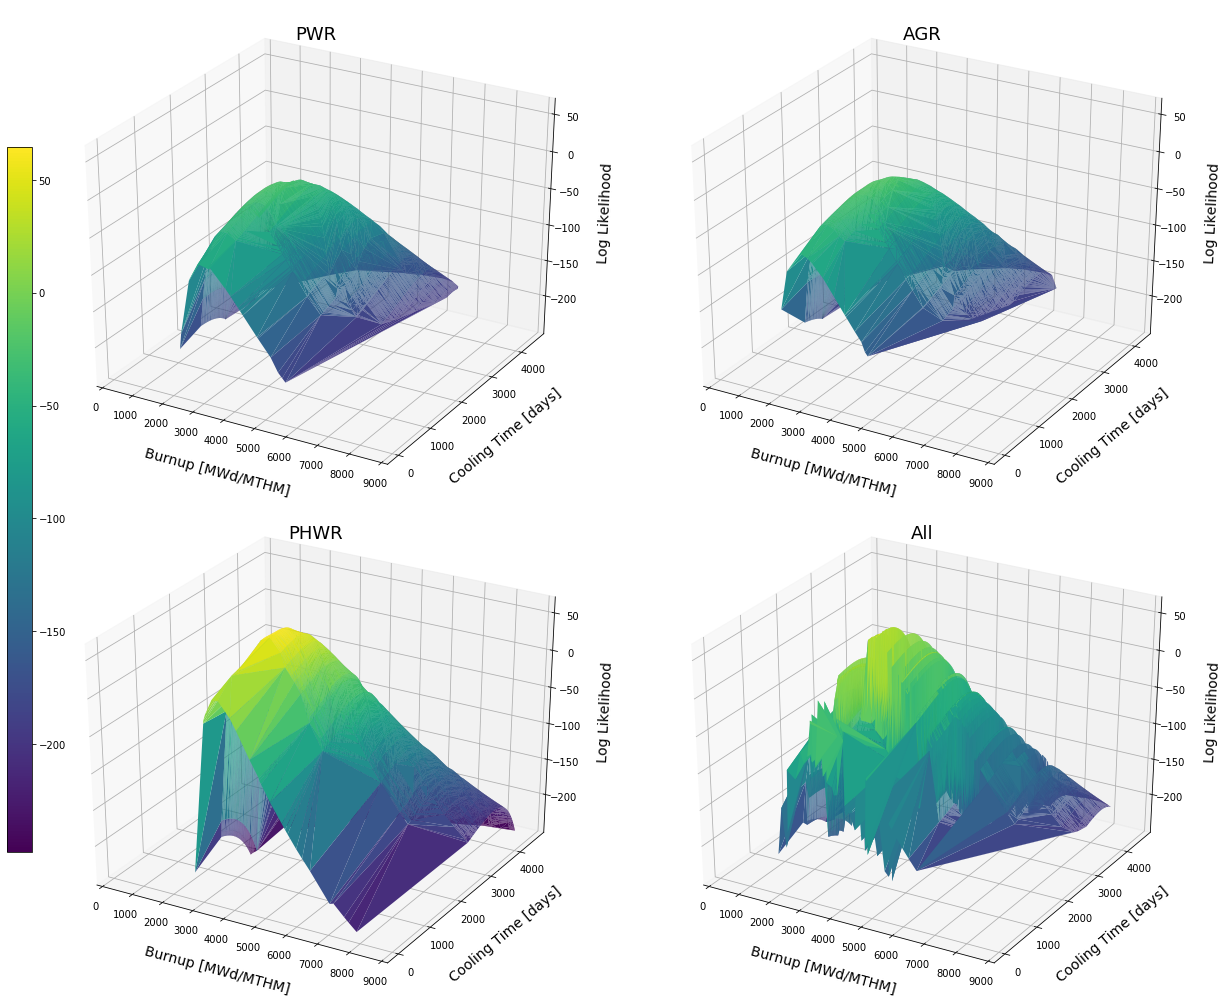
\includegraphics[height=18cm]{figures/placeholder_rxtr.png}
  \caption{placeholder figure showing filtered results wrt rxtr}
\end{minipage}%
\begin{minipage}{.5\textwidth}
  \centering
  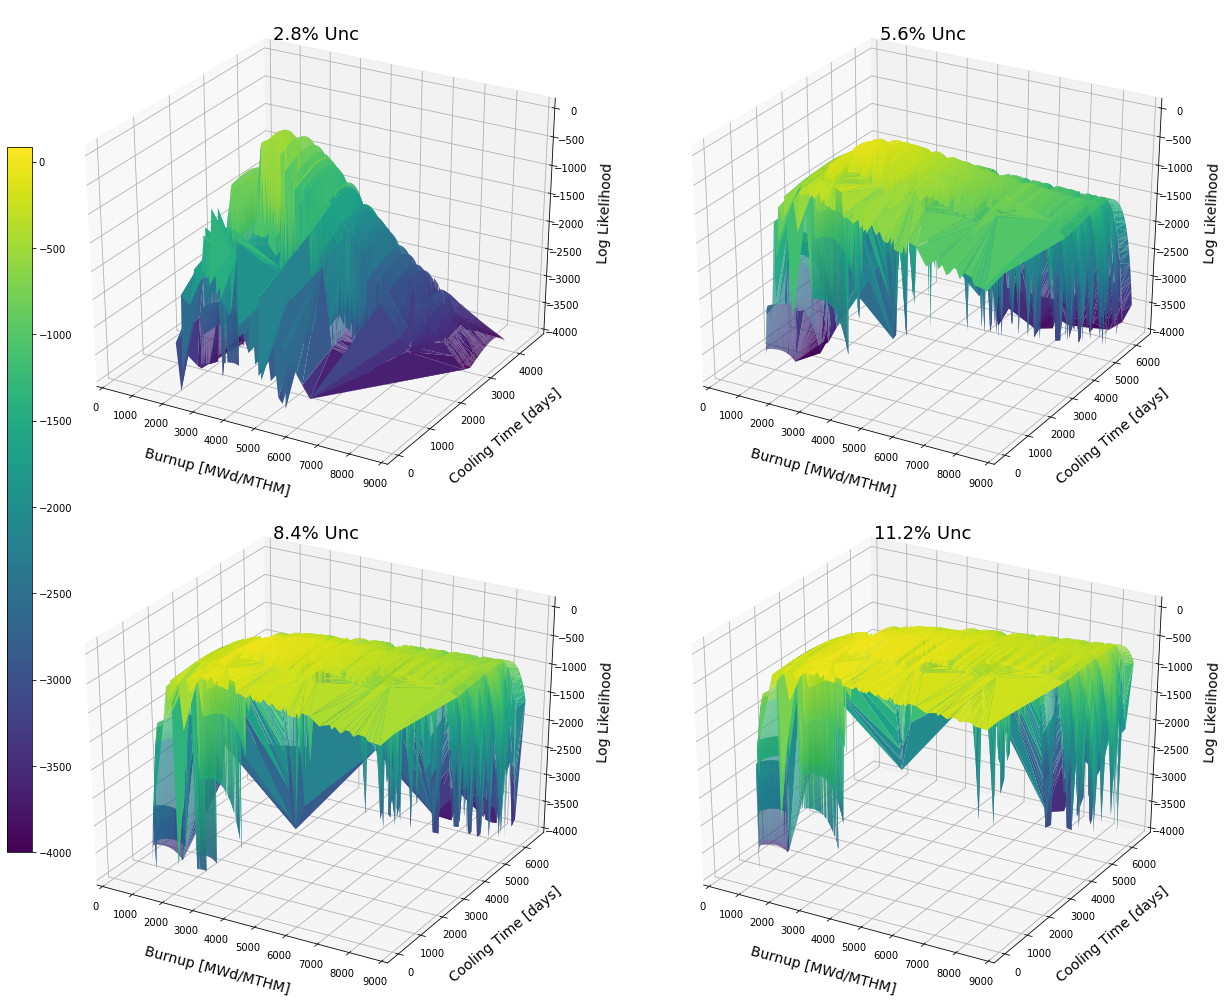
\includegraphics[height=18cm]{figures/placeholder_unc.png}
  \caption{placeholder figure showing results wrt increasing uncertainty}
\end{minipage}
\end{figure}

More texty text!

\end{block}
\end{column}

\begin{column}{0.4\textwidth}

\begin{block}{Future Work}

Information reduction using Gamma Detector and Response and Analysis Software
(GADRAS) \cite{gadras}, developed at Sandia National Laboratories, will be used
next. This limits the training set features to isotopes that are detectable
in realistic scenarios. \\~\\

Next, a real-world spent fuel database will be used for testing data: the Spent
Fuel Composition Database (SFCOMPO) \cite{sfcompo}. This will provide a
benchmark of how this method performs with measurements from commmercial
reactors worldwide. 

\end{block}

\begin{block}{References}
\printbibliography
\end{block}

\begin{block}{Funding}

\begin{minipage}{.75\textwidth}
\footnotesize
This material is based upon work supported by the U.S. Department of Homeland
Security under Grant Award Number, 2012- DN-130-NF0001. The views and
conclusions contained in this document are those of the authors and should not
be interpreted as representing the official policies, either expressed or
implied, of the U.S. Department of Homeland Security. This material is also
based upon work supported by the U.S. National Science Foundation Graduate
Fellowship Program.
\end{minipage}%
\begin{minipage}{.25\textwidth}
\begin{figure}
  \centering
  
\includegraphics[height=4.6cm]{logos/dhs.png}
  
\includegraphics[height=5.0cm]{logos/nsf.png}
\end{figure}
\end{minipage}

\end{block}

\end{column}
\end{columns}
\end{column}
\end{columns}
%%%%%%%%%%%%%%%%%%%%%%%%%%%%%%%%%%%%%%%%%%%%%%%%%%%%%%%%%%%%%%%%%%%%%%%%%%%%%%%%%%%%%%%%%%%%%%%%%%%
\end{frame}
\end{document}
